%-----------------------------------------------------------------------------
%
%               Template for sigplanconf LaTeX Class
%
% Name:         sigplanconf-template.tex
%
% Purpose:      A template for sigplanconf.cls, which is a LaTeX 2e class
%               file for SIGPLAN conference proceedings.
%
% Guide:        Refer to "Author's Guide to the ACM SIGPLAN Class,"
%               sigplanconf-guide.pdf
%
% Author:       Paul C. Anagnostopoulos
%               Windfall Software
%               978 371-2316
%               paul@windfall.com
%
% Created:      15 February 2005
%
%-----------------------------------------------------------------------------


\documentclass[preprint,10pt]{sigplanconf}

% The following \documentclass options may be useful:

% preprint      Remove this option only once the paper is in final form.
% 10pt          To set in 10-point type instead of 9-point.
% 11pt          To set in 11-point type instead of 9-point.
% numbers       To obtain numeric citation style instead of author/year.

 

\newcommand{\cL}{{\cal L}}




\usepackage[table]{xcolor}
\usepackage{hhline}

\hyphenation{op-tical net-works semi-conduc-tor}
\usepackage[linesnumbered,ruled,vlined]{algorithm2e}
\usepackage[pdftex]{graphicx}
\usepackage{siunitx}
%\usepackage{stfloats}
%\usepackage{cite}
\usepackage{amsthm}
\newtheorem*{remark}{Remark}
\usepackage{algorithmic}
\usepackage{multirow}
%\fnbelowfloat
\usepackage[tight,footnotesize]{subfigure}
\usepackage{listings}
\usepackage{color}
\usepackage{url}
\definecolor{dkgreen}{rgb}{0,0.6,0}
\definecolor{gray}{rgb}{0.5,0.5,0.5}
\definecolor{mauve}{rgb}{0.58,0,0.82}

\lstset{frame=tb,
	language=Java,
	aboveskip=3mm,
	belowskip=3mm,
	showstringspaces=false,
	columns=flexible,
	basicstyle={\small\ttfamily},
	numbers=none,
	numberstyle=\tiny\color{gray},
	keywordstyle=\color{blue},
	commentstyle=\color{dkgreen},
	stringstyle=\color{mauve},
	tabsize=3
}


\setcounter{topnumber}{10}
\setcounter{bottomnumber}{10}
\setcounter{totalnumber}{10}
\renewcommand{\floatpagefraction}{.9}
\renewcommand{\textfraction}{.2}
\DeclareGraphicsExtensions{.pdf,.png,.jpg,.mps} 



\renewcommand{\floatpagefraction}{.9}
\renewcommand{\textfraction}{.1}
\renewcommand{\topfraction}{.8}
\renewcommand{\bottomfraction}{.8}


	

\special{papersize=8.5in,11in}
\setlength{\pdfpageheight}{\paperheight}
\setlength{\pdfpagewidth}{\paperwidth}

\conferenceinfo{CONF 'yy}{Month d--d, 20yy, City, ST, Country}
\copyrightyear{20yy}
\copyrightdata{978-1-nnnn-nnnn-n/yy/mm}
\copyrightdoi{nnnnnnn.nnnnnnn}

% Uncomment the publication rights you want to use.
%\publicationrights{transferred}
%\publicationrights{licensed}     % this is the default
%\publicationrights{author-pays}


%\makeatletter
%\def\@copyrightspace{\relax}
%\makeatother
\begin{document}
 

\title{Automatic Non-functional Testing of Code Generators Families}
 

\authorinfo{Mohamed Boussaa\and Olivier Barais\and Benoit Baudry}
           {Diverse team INRIA, Rennes, France}
           { \{mohamed.boussaa, olivier.barais, benoit.baudry\}@inria.fr}
\authorinfo{Gerson Suny\'e}
           {AtlanMod team INRIA, Nantes, France}
           {gerson.sunye@inria.fr}


\maketitle

\newcommand{\etal}{et al.}
\newcommand{\eg}[0]{e.\,g.}
\newcommand{\ie}[0]{i.\,e.}

%\vspace*{-1cm}

%\boldmath
%In general, most of compiler optimizations focus on improving the execution time and performance of compiled code. However, this may be so expensive at the expense of resource usage and may induce to compiler bugs or crashes. With the increasing of resource usage, it is important to evaluate the compiler behavior. Indeed, in resource-constrained environment, compiler optimizations may lead to memory leaks or execution bottlenecks. So, a fine-grained understanding of resource consumption and analysis of compiler’s behavior regarding optimizations becomes necessary. As well, compilers may have a huge number of optimization combinations and it very hard and time-consuming to find the optimal sequence of optimization options that satisfies user key objective. In this paper, we propose DECO (Diversity-based Exploration of Compiler Optimizations), an automatic generator of compiler optimization sequences based on sequences diversity. In this approach, we apply the Novelty Search (NS) technique to determine the optimal sequence that could be used to produce a code which consumes less system resources. To do so, we explore the search space of possible optimization combinations by considering diversity of sequences as the unique objective function to be optimized. In fact, instead of having a fitness-based selection, we select optimization sequences based on a novelty score showing how different they are compared to all other solutions evaluated so far. We conduct experiments by providing a quantitative study of the impact of compiler optimizations explored by NS on non-functional properties like CPU and memory consumption. We run experiments on a commonly used set of benchmarks and we identified the optimal set of optimizations regarding performance. The results show that...
%In search-based structural testing, metaheuristic search techniques have been frequently used to automate the test data generation. In Genetic Algorithms (GAs) for example, test data are rewarded on the basis of an objective function that represents generally the number of statements or branches covered. However, owing to the wide diversity of possible test data values, it is hard to find the set of test data that can satisfy a specific coverage criterion. In this paper, we introduce the use of Novelty Search (NS) algorithm to the test data generation problem based on statement-covered criteria. We believe that such approach to test data generation is attractive because it allows the exploration of the huge space of test data within the input domain. In this approach, we seek to explore the search space without regard to any objectives. In fact, instead of having a fitness-based selection we select test cases based on a novelty score showing how different they are compared to all other solutions evaluated so far.

\begin{abstract}
The intensive use of domain specific languages (DSL) and generative programming techniques provides an elegant engineering solution to deal with the heterogeneity of platforms or technological stacks. The use of DSLs also leads to the creation of numerous code generators and compilers that will automatically translate high-level system
specifications into multi-target executable code and scripts. 
%These practices reduce clearly the development and maintenance effort by developing at a higher-level of abstraction. 
However, the use of code generators may induce different bugs and inconsistencies within generated software artifacts. Although software designers generally provide high-level test suites to verify the functional outcome of generated code, it remains challenging and tedious to verify the behavior of produced code in terms of non-functional properties.
%However, industrial code generators may have a huge number of bugs and 

This paper describes a runtime monitoring infrastructure based on system containers, as execution platform, to evaluate the consistency and coherence of generated code regarding the non-functional properties. This approach provides a fine-grained understanding of resource consumption and analysis of components behavior. 
We evaluate our approach by analyzing the non-functional properties of HAXE, a popular high-level language that involves a set of cross-platform code generators able to compile to different targets. Our initial experimental results show that our approach is able to detect non-functional bugs within HAXE code generators.
%We evaluate the effectiveness of our approach by verifying the optimizations performed by the GCC compiler, a widely used compiler in software engineering community. We also present a number of case studies, in which the tool was successfully used.

%system containers as execution platform




%they are highly dependent on target platforms
\end{abstract}
\smallskip
\noindent \textbf{Keywords.} \textit{code quality, non-functional properties, code generator, testing}.
% HD-Services will run within a heterogeneous and distributed infrastructure. To facilitate the testing of this kind of services, we need to deploy HD-services on an elastic infrastructure that provides preconfigured virtual server images, storage and network connectivity that may be provisioned by HD-Developers. Monitoring information should also be provided to inform about resource utilization required/needed and to automate the resource management. For this purpose, we propose a testing infrastructure based on docker environment. Docker will automate the deployment of applications inside software containers. It will simplify the creation of highly distributed systems by allowing multiple applications to run autonomously on a server (basically a cloud server). Docker will provide a platform as a service (PaaS) style of deployment for HD-Services. Consequently, we will rely on this technology and benefit from all its advantages to:
%1- Deploy preconfigured application to test within docker containers
%2- Automate test suites generation
%3- Monitor service containers
%4- Limit and manage resources for each running container
%5- Gather performance metrics (CPU, Memory, I/O, etc.)
%As a consequence, we are going to integrate a collection of docker technologies to define the adequate infrastructure for testing HD-Services.



%In model-driven engineering, developers use different code generators to translate source programs represented in a graphical modeling language into general purpose programming languages such as C, Java, C++,etc.  These code generators serve as a basis to target different ranges of platforms. Many technologies, such as Docker containers, provide new opportunities to automate the deployment of produced code into a distributed and heterogeneous component-based infrastructure. In fact, during the code generation process, different optimizations may be applied for code transformation. For example, embedded systems for which code is generated often have limited resources. Therefore, optimization techniques must be applied whenever possible to generate efficient code with respect to memory consumption, execution time, disk writing speed, among others. Sometimes, optimizations can even lead to memory leaks or execution bottlenecks especially for resource-constrained systems. So, to ensure the efficiency of generated code, deployed components must be checked and verified regarding their non-functional behavior. This paper describes a component-based tool for testing and monitoring generated code. It provides a fine-grained understanding of resource consumption and analysis of components behavior regarding optimizations. We evaluate the effectiveness of our test approach by means of testing optimizations performed by the GCC compiler, a widely used compiler in software engineering community. We present as well a number of case studies, in which the tool was successfully used.

%\vfill


%\vspace*{-2cm}
\section{Introduction}
In model-driven software engineering, the intensive use of generative programming techniques has become a common practice for software development since it reduces the development and maintenance effort by developing at a higher-level of abstraction through the use of domain-specific languages~\cite{brambilla2012model} (DSLs). 
DSLs, as opposed to general-purpose languages, are software languages that focus on specific problem domains. Thus, the realization of model-driven software development for a specific domain requires the creation of effective code generators and compilers for these DSLs.
The use of code generators is needed to transform manually designed models to software artifacts, which can be deployed on different target platforms. 
Code-generation environments automate and systematize the process of building
families of software systems which can clearly reduce the effort of software implementation. In fact, a code generator is able to translate source code programs represented in a graphical/textual modeling language (model) into general purpose programming languages such as C, Java, C++, etc. In turn, generated code is transformed into machine code (binaries) using a set of specific compilers.
These compilers serve as a basis to target different ranges of platforms. 
%Many technologies, such as Docker containers, provide new opportunities to automate the deployment of produced code into a distributed and heterogeneous component-based infrastructure
However, code generators can be difficult to understand since they involve a set of complex and heterogeneous technologies which make the task of performing design, implementation, and maintenance very hard and time-consuming[ref]. Generally, in order to check the correctness of code generation process, developers often use to define (at design time) a set of test cases that verify the functional outcome of generated code. Afterwards, test cases are executed within each specific target platform which can lead to either a correct behavior or a failure (e.g., crashes, bugs). 
For non-functional testing of code generators, developers need to deploy and execute software artifacts within different execution platforms. Then, they have to collect and visualize information about the performance and efficiency of generated code. Finally, they report issues related to the code generation process such as incorrect typing, memory management leaks. etc. To do so, developers general use several platform-specific profilers and monitoring tools in order to find some inconsistencies or bugs during code execution. Ensuring the code quality of generated code can refer to several non-functional properties such as code size, resource or energy consumption, execution time, among others [ref]. Therefore, testing the non-functional properties remains challenging and time-consuming task because developers have to analyze and verify code for each target platform using platform dependent tools.




%In fact, during the code generation process, different optimizations may be applied for code transformation. Improvement of source program can refer to several different characteristics of the produced code such execution time, memory consumption, code size, among others~\cite{almagor2004finding,pan2006fast}.
%For example, embedded systems for which code is generated often have limited resources. 
%\begin{figure}[h]
%	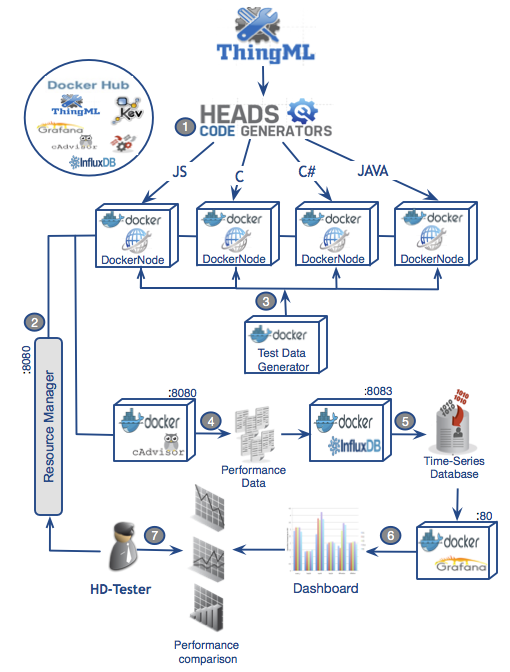
\includegraphics[width=1.\linewidth]{Ressources/app.png}
%	\caption{Overview of the Docker-based testing architecture}
%\end{figure}




%Model-based code generators integrate rule-based model-to-model transformation languages such as ATL and template-based model-to-text transformation languages such as Acceleo to translate high-level system specifications into executable code and scripts. A








\cleardoublepage
Therefore, optimization techniques must be applied whenever possible to generate efficient code with respect to available resources\cite{nagiub2013automatic}. 
As general-purpose optimizations, compiler creators\footnote{We consider compilers as a kind of code generators in this paper. Indeed, from the testing point of view, we do not make any differences between testing code generators and testing compilers} usually define fixed and program-independent sequence optimizations.
For example, in GCC, we can distinguish optimization levels from O1 to O3. Each optimization level involves a fixed list of compiler optimization options. 
However, industrial code generators may have a huge number of potential optimization combinations, making it hard and time-consuming for software developers to find the sequence of optimizations that satisfies user key objectives. 

In this paper we explore the relationship between runtime execution of optimized code and non-functional properties.
We propose a component-based tooled approach to check code generators non-functional properties through the monitoring of generated code in a controlled sandboxing environment. 
Our approach is based on microservices to automate the deployment and monitoring of different variants of optimized code into a distributed and heterogeneous component-based infrastructure. 
We assess the effectiveness of our approach by evaluating the optimizations performed by the GCC compiler, a widely used compiler in software engineering community. 
We also present a number of case studies, in which the tool was successfully used.
%This to ensure the efficiency of generated code, deployed components must be checked and verified regarding their non-functional behavior
%\footnote{\url{https://www.docker.com}} 

The primary contribution of this paper can be summarized as follows: 
(1) We propose a microservice infrastructure to ensure the deployment and monitoring of generated code regarding resource consumption; 
(2) We evaluate the effectiveness of our approach by testing the GCC compiler optimizations across two case studies.
 

The paper is organized as follows.
Section II describes the motivation behind this work. A search-based technique for compiler optimizations exploration is presented in Section III. 
We present in Section IV our infrastructure for non-functional testing using microservices. 
The evaluation and results of our experiments across two case studies are discussed in Section V. 
Finally, related work, concluding remarks and future work are provided in Sections VI and VII.


%The difference between classical compilers like GCC, LLVM and code generators is that code generators are used only by few people comparing to famous compilers like GCC. Moreover, code generators face a high rate of changes and update versions due to new development needs. Hence, it becomes necessary to check the quality of produced code. This will help software maintainers to verify the correct functioning of code generators.  Among the most important properties to check, we distinguish the non functional properties.

%Like traditional compilers, code generators typically perform multiple passes over various intermediate forms during code transformation. Many rules may also be applied and that differs from one generator to another. These passes are complex and highly dependent on target platform architecture. 

 
 

  % \section{Motivations}
 %\section{Previous work}
%\section{Approach Overview}

\section{Motivation}

A reliable and accepted way to increase confidence in the correct functioning of code generators is to validate and check the functionality of generated code, which is common practice for compiler validation and testing.
Therefore, developers try to check the syntactic and semantic correctness of generated code by means of different techniques such as static analysis, test suites, etc., and ensure that the code is behaving correctly. 
In model-based testing, testing code generators focuses on testing the generated code against its design. Thus, the model and the generated code are executed in parallel, by means of simulations, with the same set of test suites. Afterwards, the two outputs are compared with respect to certain acceptance criteria. Test cases, in this case, can be designed to maximize the code or model coverage. [ref back to back testing/systematic]


Another important aspect of code generator's testing is to test the non-functional properties of produced code. Proving that the generated code is functionally correct is not enough to claim the effectiveness of the code generator under test. 
In fact, code generators have to respect different requirements which preserve software reliability and quality. A non-efficient code generator might generate defective software artifacts (code smells) that violates common software engineering practices. Thus, poor-quality code can affect system reliability and performance (e.g., high resource usage, low execution speed, etc.).


Figure 1 shows an overall overview of the different processes that are involved together to ensure the code generation and non-functional testing of produced code from design time to run time. We distinguish 4 major steps: the software design using high-level system specifications, code generation by means of code generators, code execution, and non-functional testing of generated code. 

So first, software developers have to create, at design time, new models that describe software's behavior using a high-level design language, generally DSLs. Afterwards, developers can use platform-specific code generators to ease the software development and generate automatically code that targets different languages and platforms. We depict, in Figure 1, three code generators capable to generate code in three software programming languages (JAVA, C\# and C++). In this step, the code generator takes as an input the previously designed model and produce, as a consequence, software artifacts for the desired target platform. Transformations from model to code within each code generator might be different and may integrate different transformation rules. As an example, we distinguish model-to-model transformations languages such as ATL[ref] and template-based model-to-text transformation languages such as Acceleo [ref] to translate high-level system specifications into executable code and scripts [ref WS]. The main task of code generators is to transform models to general-purpose and platform-dependent languages. In the next step, generated software artifacts (e.g., JAVA, C\#, C++, etc.) with their generated test suites are compiled, deployed and executed across different target platforms (e.g., Android, ARM/Linux, JVM, x86/Linux, etc.). Thus, several code compilers are needed to transform source code to machine code (binaries) in order to get executed. 
Finally, to perform the non-functional testing of generated code, developers have to collect and visualize information about the performance and efficiency of running code across the different platforms. 
Therefore, they generally use several platform-specific profilers, trackers, instrumenting and monitoring tools in order to find some inconsistencies or bugs during code execution. Ensuring the code quality of generated code can refer to several non-functional properties such as code size, resource or energy consumption, execution time, among others. Finding inconsistencies within code generators involves analyzing and inspecting the code and that, for each execution platform. For example, one of the solutions is to analyze the memory footprint of software execution and find memory leaks. Developers then, can inspect the source code and find some parts of the code-base that have triggered this issue. Such non-functional error could occur when the code generator produces code that presents for example: incorrect typing, faulty memory management, code-smells, etc. Therefore, software testers generally use to report statistics about the performance of generated code in order to fix, refactor, and optimize the code generation process.

In short, then, we believe that testing the non-functional properties of code generators remains challenging and time-consuming task because developers have to analyze and verify code for each target platform using platform-dependent tools which makes the task of maintaining code generators very tedious. The heterogeneity of platforms and the diversity of target software languages increase the need of supporting tools that can evaluate the consistency and coherence of generated code regarding the non-functional properties. This paper describes a new approach, based on micro-services as execution platforms, to automate and ease the non-functional testing of code generators. This runtime monitoring infrastructure provides a fine-grained understanding of resource consumption and analysis of generated code's behavior.



 




\iffalse 
//footprint
//It is also possible to automatically generate test suites for software artfacts 
//model coverage
//System resources and architecture of each execution platform might vary 
//talk about platform specific profilers
//heterogeneous execution platforms
//the need of system level abstraction/virtualization to handle heterogeneity
//ease the monitoring process 
//add figure of SOTA 
\fi




\cleardoublepage
\iffalse 
\subsection{Compilers Optimizations}
In the past, researchers have shown that the choice of optimization sequences may impact software performance~\cite{almagor2004finding,chen2012deconstructing}. 
As a consequence, software-performance optimization becomes a key objective for both, software industries and developers, which are often willing to pay additional costs to meet specific performance goals, especially for resource-constrained systems.

Universal and predefined sequences, \eg, O1 to O3 in GCC, may not always produce good performance results and may be highly dependent on the benchmark and the source code they have been tested on~\cite{almagor2004finding,hoste2008cole}.
Indeed, each one of these optimizations interacts with the code and in turn with all other optimizations in complicated ways. Similarly, code transformations can either create or eliminate opportunities for other transformations and it is quite difficult for users to predict the effectiveness of optimizations on their source code program.
As a result, most software engineering programmers that are not familiar with compiler optimizations find difficulties to select effective optimization sequences.

To explore the large optimization space, users have to evaluate the effect of optimizations and optimization combinations, for different target platforms. 
Thus, finding the optimal optimization options for an input source code is a challenging, very hard, and time-consuming problem. 
Many approaches~\cite{hoste2008cole,zhong2009tuning,sandran2012genetic,martins2014exploration} have attempted to solve this optimization selection problem using techniques such as genetic algorithms, iterative compilation, etc.

%problem
It is important to notice that performing optimizations to source code can be so expensive at the expense of resource usage and may induce to compiler bugs or crashes. 
%With the increasing of resource usage, it is important to evaluate the compiler behavior. 
Indeed, in a resource-constrained environment and because of insufficient resources, compiler optimizations can even lead to memory leaks or execution crashes~\cite{yang2011finding}. 
Thus, a fine-grained understanding of resource consumption and analysis of compilers behavior regarding optimizations becomes necessary to ensure the efficiency of generated code.

\subsection{Example: GCC Compiler}

The GNU Compiler Collection, GCC, is a very popular collection of programming compilers, available for different platforms.
GCC exposes its various optimizations via a number of flags that can be turned on or off through command-line compiler switches. 
The diversity of available optimization options makes the design space for optimization level very huge, increasing the need for heuristics to explore the search space of feasible optimizations sequences.

% We choose GCC compiler as a motivating example in order to explain how we would study the impact of compiler optimizations using a component-based infrastructure for testing and monitoring.
% In next section, we present a search-based technique called Novelty Search for automatic generation of optimization sequences.

For instance, version 4.8.4 provides a wide range of command-line optimizations that can be enabled or disabled, including more than 150 options for optimization. 
Table I summarizes the optimization flags that are enabled by the default optimization levels O1 to O3.
We count 76 optimization flags, resulting in a huge space with $2^{76}$ possible optimization combinations.
In our approach, we did not consider some optimization options that are enabled by default, since they do not affect the performance of generated binaries.
Optimization flags in GCC can be turned off by using "fno-"+flag instead of "f"+flag in the beginning of each optimization. 
We use this technique to play with compiler switches.

\begin{table}
	\label{table:options}
	\centering
	\caption{Compiler optimization options within standard optimization levels}
	\scalebox{0.88}{
		\begin{tabular}[c]{|c|p{3cm}||c|p{3cm}|}
			
			
			\cline{1-4}
			Level & Optimization option & Level & Optimization option  \\
			\hline
			O1 & 
			-fauto-inc-dec \newline
			-fcompare-elim \newline
			-fcprop-registers \newline
			-fdce \newline
			-fdefer-pop \newline
			-fdelayed-branch \newline
			-fdse \newline
			-fguess-branch-probability \newline
			-fif-conversion2 \newline
			-fif-conversion \newline
			-fipa-pure-const \newline
			-fipa-profile \newline
			-fipa-reference\newline 
			-fmerge-constants\newline
			-fsplit-wide-types \newline
			-ftree-bit-ccp \newline
			-ftree-builtin-call-dce \newline
			-ftree-ccp \newline
			-ftree-ch \newline
			-ftree-copyrename \newline
			-ftree-dce \newline
			-ftree-dominator-opts \newline
			-ftree-dse \newline
			-ftree-forwprop \newline
			-ftree-fre \newline
			-ftree-phiprop \newline
			-ftree-slsr \newline
			-ftree-sra \newline
			-ftree-pta \newline
			-ftree-ter \newline
			-funit-at-a-time
			
			&
			\multirow{2}{*}{O2} & \multirow{2}{6cm} {
				-fthread-jumps\newline 
				-falign-functions\newline  
				-falign-jumps \newline
				-falign-loops  \newline
				-falign-labels \newline
				-fcaller-saves \newline
				-fcrossjumping \newline
				-fcse-follow-jumps  \newline
				-fcse-skip-blocks \newline
				-fdelete-null-pointer-checks \newline
				-fdevirtualize \newline
				-fexpensive-optimizations \newline
				-fgcse  \newline
				-fgcse-lm  \newline
				-fhoist-adjacent-loads \newline
				-finline-small-functions \newline
				-findirect-inlining \newline
				-fipa-sra \newline
				-foptimize-sibling-calls \newline
				-fpartial-inlining \newline
				-fpeephole2 \newline
				-fregmove \newline
				-freorder-blocks  \newline
				-freorder-functions \newline
				-frerun-cse-after-loop \newline 
				-fsched-interblock \newline 
				-fsched-spec \newline
				-fschedule-insns  \newline
				-fschedule-insns2 \newline
				-fstrict-aliasing \newline
				-fstrict-overflow \newline
				-ftree-switch-conversion\newline -ftree-tail-merge \newline
				-ftree-pre \newline
				-ftree-vrp
			} \\
			\cline{1-2}
			O3 & 
			-finline-functions \newline
			-funswitch-loops\newline
			-fpredictive-commoning \newline
			-fgcse-after-reload \newline
			-ftree-vectorize \newline
			-fvect-cost-model \newline
			-ftree-partial-pre \newline 
			-fipa-cp-clone  & &  \\
			\cline{1-2}
			Ofast & -ffast-math &   &  \\
			\hline
			
		\end{tabular}
	}
\end{table}
\fi
%\section{Novelty Search Compiler Optimizations Exploration}
 
The goal of the novelty search approach for compiler optimization, introduced by Lehman and Stanley in 2008
[22], is to identify a set of compiler optimization levels that provide a trade-off with respect to resource utilization. 

\subsection{Novelty Search Adaptation}
Optimization options are difficult and even impossible to be chosen by programmers or compiler users. So a tool to help users to choose the best set of options becomes necessary to achieve a compiler optimization with effectiveness and efficiently. 

There have been many previous works that have investigated this problem by using different techniques like search based or machine learning techniques, among others[ref]. Some of the works focused on optimizing compilers in term of execution time. Some others focused on reducing the energy consumption of running programs on hardware machines.

In this work, we aim to provide a new alternative for choosing effective compiler optimization options. In fact, since the search space of possible combinations is too large, we aim to use a new search based technique called Novelty Search to tackle this issue. The idea of this approach is to explore the search space of possible compiler flag options without regard to any objective. In fact, instead of having a fitness-based selection that aim to optimize either execution time or energy consumption, we select optimization sequences based on a novelty score showing how different they are compared to all other combinations evaluated so far. This makes the tool fitness and program independent.

We think also that the search toward effective optimization sequences is not straightforward since the interactions between optimizations is too complex and difficult to predict and to define. In a previous work for example, Chen et al. \cite{chen2012deconstructing}showed that a handful optimizations may lead to higher speedup than other techniques of iterative optimization. In fact, the fitness-based search may be trapped into some local optima that can not escape. This phenomenon is known as "diversity loss". For example, if the most effective optimization sequence that induces less execution time, lies far from the search space defined by the gradient of the fitness function, then some promising search areas may not be reached. The issue of premature convergence to local optima has been a common problem in evolutionary algorithms. Many methods are proposed to overcome this
problem. However, all these alternatives use a fitness-based selection to guide the search. 
Therefore, diversity maintenance in the population level is key for avoiding premature convergence. Considering diversity as the unique objective function to be optimized may be a key solution to this problem.

So during the evolutionary process, we use to select optimization sequences that remain in sparse regions of the search space in order to guide the search through novelty. In the meanwhile, we choose to gather non-functional metrics of explored sequences namely memory and CPU consumption. These metrics will provide us a more fine-grained understanding and analysis of compiler's behavior regarding optimizations. 
\begin{algorithm}
	\caption{Novelty search algorithm for compiler optimizations exploration}
	\label{alg1}
	\begin{algorithmic}[1]
		\REQUIRE Optimization sequences S
		\REQUIRE Benchmark programs Benchmark
		
		\REQUIRE Novelty threshold T
		\REQUIRE Limit L
		\REQUIRE Nearest neighbors K
		
		\ENSURE Best optimization sequence best\_sequence
		\STATE $initialize\_archive(archive,L)$
		\STATE $population \gets random\_sequences(S)$
		\REPEAT
		
		\FOR{$sequence \in population$}   
		\FOR{$program \in benchmark$}
		\STATE 	$perfomance \gets execute(sequence,program)$
		\ENDFOR
		\STATE	$novelty\_metric(sequence) \gets distFromKnearest(archive,population,K)$
		
		\IF{$novelty\_metric > T$}
		\STATE	$archive \gets archive \cup sequence$
		\ENDIF
		
		\ENDFOR
		
		\STATE		$new\_population \gets generate\_new\_population(population)$
		\STATE		$generation \gets generation + 1$
		\UNTIL{generation = N}
		\RETURN best\_sequence
	\end{algorithmic}
\end{algorithm}
\subsubsection{Optimization sequences representation}
For our case study, a candidate solution represents all compiler switches that are used in the 4 standard optimization levels (O1, O2, O3 and Ofast). Thereby, we represent this solution as a vector where each dimension is a compiler flag. The variables which represent compiler options are represented as genes in a chromosome. So, a solution represents the CFLAGS value used by GCC to compile programs.
A solution has always the same size which is the total number of involved flags. But, during the evolutionary process, these flags are turned on or off depending on the mutation and crossover operators. As well, we keep the same order of invoking compiler flags since that does not affect the optimization process and it is handled internally by GCC.

\subsubsection{Novelty Metric}
The Novelty metric expresses the sparseness of an input optimization sequence. It measures its distance to all other sequences in the current population and to all sequences that were discovered in the past (i.e., sequences in the archive).
This measure expresses how unique the optimization sequence is. We can
quantify the sparseness of a solution as the average
distance to the k-nearest neighbors. If the average distance to
a given point's nearest neighbors is large then it belongs to
a sparse area and will get a high novelty score. Otherwise,
if the average distance is small so it belongs certainly to
a dense region then it will get a low novelty score. The distance between two sequences is computed as the total number of symmetric differences among optimization options. Formally, we define this distance as follows :
\begin{equation}
distance(S1,S2)=\left | S1 \bigtriangleup S2 \right |
\end{equation}
where $S1$ et $S2$ are two selected optimization sequences (solutions), In this equation, we calculate the cardinality of the symmetric difference between the two sequences. This distance will be 0 if two optimization sequences are similar and higher than 0 if there is at least one optimization difference. The maximum distance is equal to the total number of input flags.

To measure the sparseness of a solution, we will use the previously defined distance to compute the average distance of a sequence to its k-nearest neighbors. In this context, we define the novelty metric of a particular solution as follows:
\begin{equation}
NM(S) = \frac{1}{k} \sum_{i=1}^{k} distance(S,\mu _{i})
\end{equation}
where $\mu _{i}$ is the $i^{th}$ nearest neighbor of the solution S within the population and the archive of novel individuals.
\section{Approach Overview}


\subsection{Non-Functional Testing of a Code Generator Family: a Common Process}

Figure 1 summarizes the classical steps to ensure the code generation and non-functional testing of produced code from design time to run time. 
We distinguish 4 major steps: the software design using high-level system specifications, code generation by means of code generators, code execution, and non-functional testing of generated code. 


\begin{figure*}[t]
	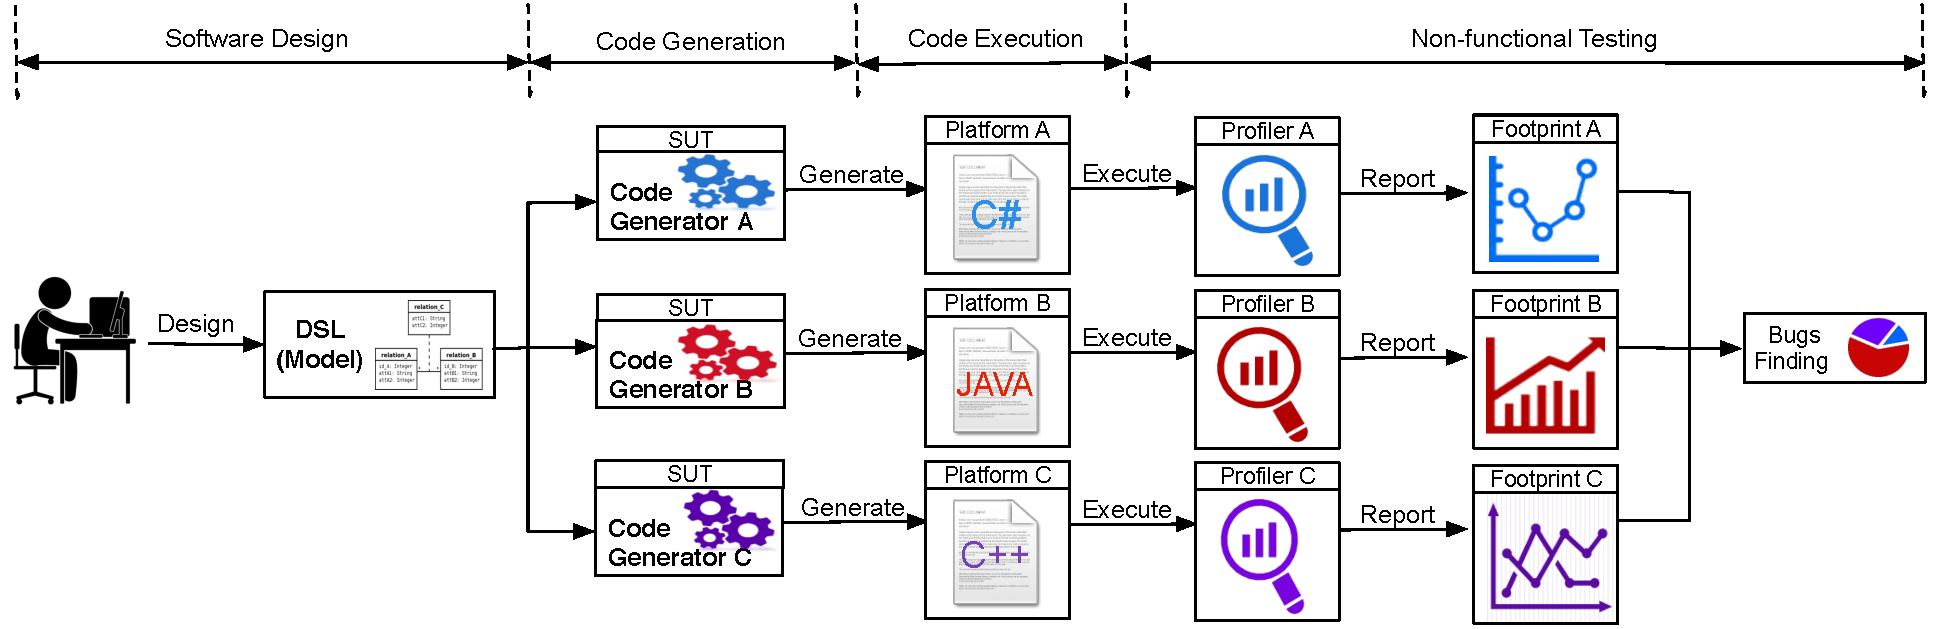
\includegraphics[width=1\linewidth]{Ressources/background.pdf}
	\caption{An overall overview of the different processes involved to ensure the code generation and non-functional testing of produced code from design time to run time: the classical way}
	%		\label{AAA}
\end{figure*}


In the first step, software developers have to define, at design time, software's behavior using a high-level abstract language (DSLs, models, program, etc). Afterwards, developers can use platform-specific code generators to ease the software development and generate automatically code that targets different languages and platforms. We depict, in Figure 1, three code generators capable to generate code in three software programming languages (JAVA, C\# and C++). In this step, code generators transform the previously designed model to produce, as a consequence, software artifacts for the target platform.

% Transformations from model to code within each code generator might be different and may integrate different transformation rules. As an example, we distinguish model-to-model transformations languages such as ATL~\cite{jouault2005transforming} and template-based model-to-text transformation languages such as Acceleo~\cite{musset2006acceleo} to translate high-level system specifications into executable code and scripts~\cite{bragancca2008transformation,czarnecki2003classification}. The main task of code generators is to transform models to general-purpose and platform-dependent languages.
In the next step, generated software artifacts (e.g., JAVA, C\#, C++, etc.) are compiled, deployed and executed across different target platforms (e.g., Android, ARM/Linux, JVM, x86/Linux, etc.). Thus, several code compilers are needed to transform source code to machine code (binaries) in order to get executed. 

Finally, to perform the non-functional testing of generated code, developers have to collect, visualize and compare information about the performance and efficiency of running code across the different platforms. 
Therefore, they generally use several platform-specific profilers, trackers, instrumenting and monitoring tools in order to find some inconsistencies or bugs during code execution~\cite{guana2014chaintracker,delgado2004taxonomy}. Ensuring the code quality of generated code can refer to several non-functional properties such as code size, resource or energy consumption, execution time, among others~\cite{pan2006fast}. Finding inconsistencies within code generators involves analyzing and inspecting the code and that, for each execution platform. For example, one of the methods to handle that is to analyze the memory footprint of software execution and find memory leaks. Developers can then inspect the generated code and find some parts of the code-base that have triggered this issue. %Such non-functional error could occur when the code generator produces code that presents for example: incorrect typing, faulty memory management, code-smells, etc. 
Therefore, software testers generally use to report statistics about the performance of generated code in order to fix, refactor, and optimize the code generation process. Our approach aims to automate the three last steps: generate code for a set of platforms, execute code on top of different platforms, monitor and compare the execution. 

\subsection{An Infrastructure for Non-functional Testing Using System Containers}
To assess the performance/non-functional properties of generated code many system configurations (i.e., execution environments) must be considered. Running different applications (i.e., generated code) with different configurations on one single machine is complex  a single system has limited resources and this can lead to performance regressions. Moreover, each execution environment comes with a collection of appropriate tools such as compilers, code generators, debuggers, profilers, etc. Therefore, we need to deploy the test harness, \ie the produced binaries, on an elastic infrastructure that provides to compiler user facilities to ensure the deployment and monitoring of generated code in different environment settings. 

Consequently, our infrastructure provides support to automatically:
\begin{enumerate}
	\item Deploy the generated code, its dependencies and its  execution environments
	\item Execute the produced binaries in an isolated environment 
	\item Monitor the execution 
	\item Gather performance metrics (CPU, Memory, etc.)
\end{enumerate}

To get these four main steps, we rely on system containers~\cite{soltesz2007container}. Thus, instead of configuring all code generators under test (GUTs) within the same host machine, we wrap each GUT within a system container. Afterwards, a new instance of the container is created to enable the execution of generated code in an isolated and configured environment. Meanwhile, we start our runtime testing components. A monitoring component collects usage statistics of all running containers and save them at runtime in a time series database component. Thus, we can compare later informations about the resource usage of generated programs and detect inconsistencies within code generators.


The rest of this section details the technical choices we have made to synthesize this testing infrastructure.

\subsection{Technical Implementation}

The general overview of the technical implementation is shown in Figure 2. In the following subsections, we describe the deployment and testing architecture of generated code using system containers.


\begin{figure*}[!h]
	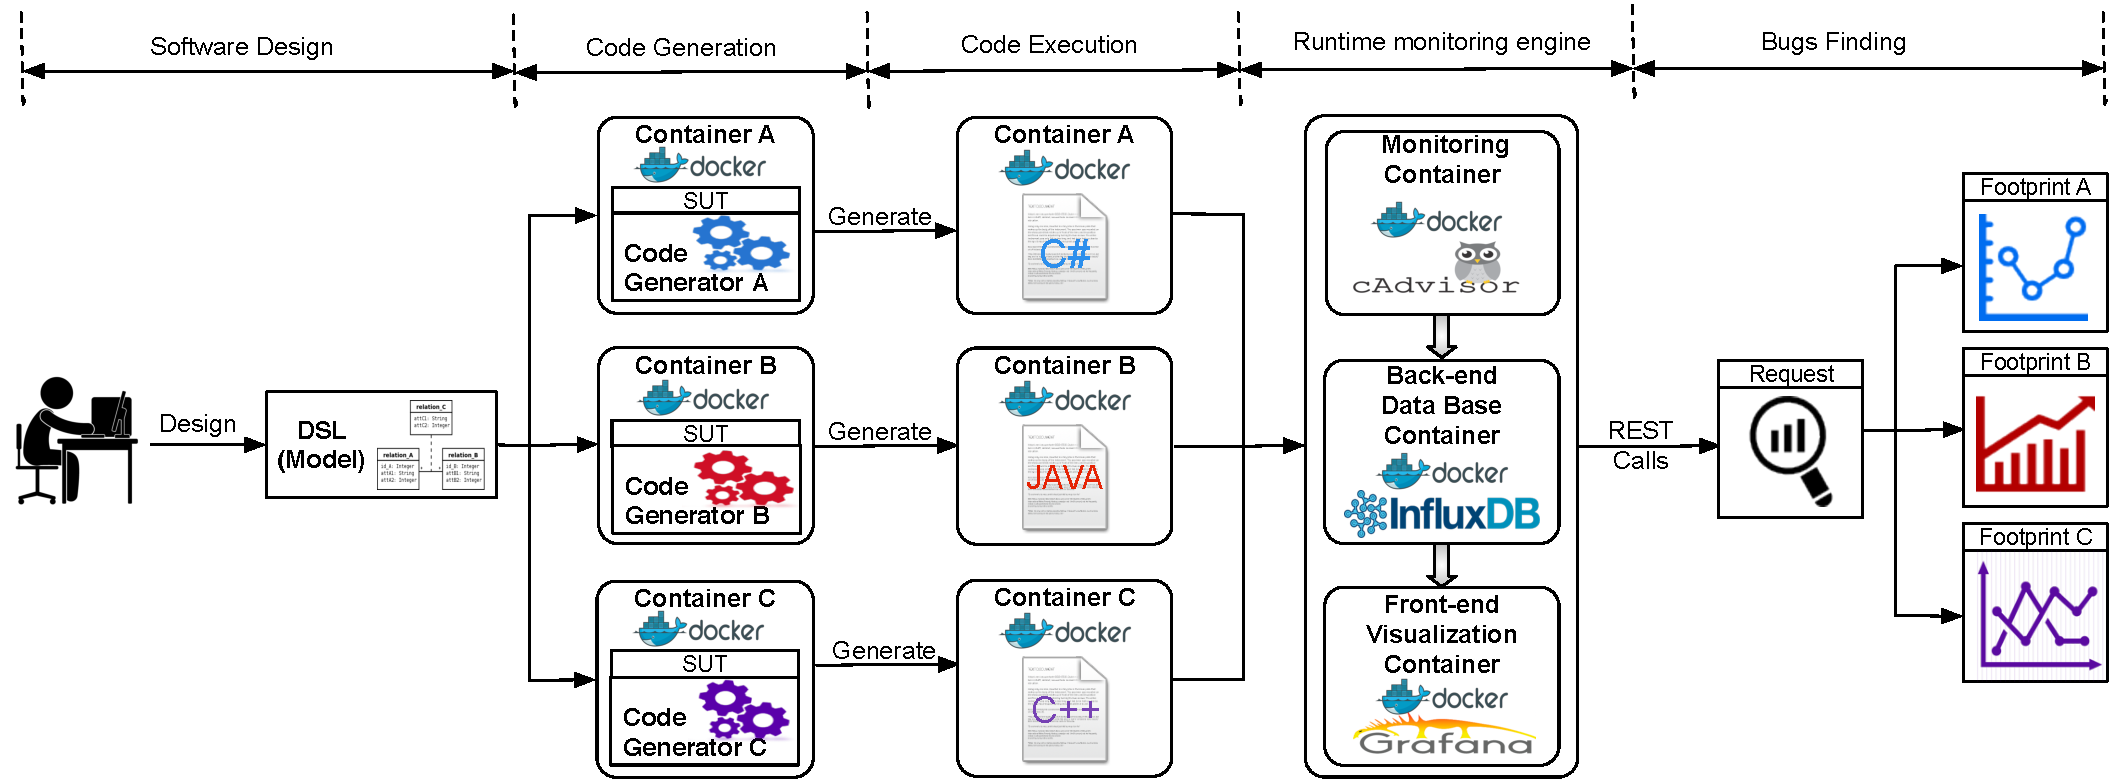
\includegraphics[width=1\linewidth]{Ressources/background2.pdf}
	\caption{A technical overview of the different processes involved to ensure the code generation and non-functional testing of produced code from design time to runtime.}
	%		\label{AAA}
\end{figure*}


\subsubsection{System Containers as Execution Platforms}


%For this purpose, we propose a testing infrastructure based on System Container techniques such as Docker\footnote{\url{https://www.docker.com}} environment. 
%This framework automates the deployment and execution of applications inside software containers by allowing multiple program configurations to run autonomously on different servers (i. e., a cloud servers).
%It also provides a distributed environment where system storage and resources can be finely managed and limited according to the needs. 

%Thus, we integrate a collection of components to define the adequate infrastructure for testing and monitoring of code generators. 


Before starting to monitor and test applications, we have to deploy generated code on different components to ease containers provisioning and profiling. 
We aim to use Docker Linux containers to monitor the execution of different generated artifacts in terms of resource usage~\cite{merkel2014docker}. 
Docker\footnote{\url{https://www.docker.com}} is an engine that automates the deployment of any application as a lightweight, portable, and self-sufficient container that runs virtually on a host machine. 
%To achieve that, Docker uses the Linux container technology. 
Using Docker, we can define pre-configured applications and servers to host as virtual images. We can also define the way the service should be deployed in the host machine using configuration files called Docker files. 
In fact, instead of configuring all code generators under test (GUTs) within the same host machine (as shown in Figure 1), our tool wrap each GUT within a container. To do so, we create a new configuration image for each GUT (i.e., the Docker image) where we install all the libraries, compilers, and dependencies needed to ensure the code generation and compilation. Thereby, the GUT produce code within multiple instances of preconfigured Docker images (see code generation step in Figure 2).
%As properties, we can define the OS where the service has to run, dependencies, etc. 
%A simple way to build images automatically is to use Dockerfiles which represents configuration files.
%Docker can build images automatically by reading the instructions from a Dockerfile. 
We use the public Docker registry\footnote{\url{https://hub.docker.com/}} for  saving, and managing all our Docker images. 
%It represents a cloud-based registry service for building and shipping application or service containers.
We can then instantiate different containers from these Docker images. 
%Basically, each container deploys an optimized version of the input source code program.

Next, each generated code is executed individually inside an isolated Linux container (see code execution step in Figure 2). By doing so, we ensure that each executed program runs in isolation without being affected by the host machine or any other processes. Moreover, since a container is cheap to create, we are able to create too many containers as long as we have new programs to execute.  
Since each program execution requires a new container to be created, it is crucial to remove and kill containers that have finished their job to eliminate the load on the system. We run the experiment on top of a private data-center that provide a bare-metal installation of  docker and docker swarm. On a single machine,  containers/softwares are running sequentially and we pin $p$ cores and $n$ Gbytes of memory for each container\footnote{$p$ and $n$ can be cofigured}. Once the execution is done, resources reserved for the container are automatically released to enable spawning next containers. Therefore, the host machine will not suffer too much from performance trade-offs.

In short, the main advantages of this approach are:
\begin{itemize}
	\item The use of containers induces less performance overhead and resource isolation compared to using a full stack virtualization solution~\cite{spoiala2016performance}. Indeed, instrumentation and monitoring tools for memory profiling like Valgrind~\cite{nethercote2007valgrind} can induce too much overhead.
	\item Thanks to the use of Dockerfiles, the proposed framework can be  configured by software testers in order to define the code generators under test (\eg, code generator version, dependencies, etc.), the host IP and OS, the DSL design, the optimization options, etc. Thus, we can use the same configured Docker image to execute different instances of generated code. For hardware architecture, containers share the same platform architecture as the host machine (e.g., x86, x64, ARM, etc.). 
	\item Docker uses Linux control groups (Cgroups) to group processes running in the container. This allows us to manage the resources of a group of processes, which is very valuable. 
	This approach increases the flexibility when we want to manage resources, since we can manage every group individually. For example, if we would evaluate the non-functional requirements of generated code within a resource-constraint environment, we can  request and limit resources within the execution container according to the needs.
	\item Although containers run in isolation, they can share data with the host machine and other running containers. Thus, non-functional data relative to resource consumption can be gathered and managed by other containers (\ie, for storage purpose, visualization)
\end{itemize}




\subsubsection{Runtime Testing Components}
In order to test our running applications within Docker containers, we aim to use a set of Docker components to ease the extraction of resource usage information (see runtime monitoring engine in Figure 2).
\paragraph{Monitoring Component}
This container provides an understanding of the resource usage and performance characteristics of our running containers. Generally, Docker containers rely on Cgroups file systems to expose a lot of metrics about accumulated CPU cycles, memory, block I/O usage, etc. Therefore, our monitoring component automates the extraction of runtime performance metrics stored in Cgroups files. For example, we access live resource consumption of each container available at the Cgroups file system via stats found in \textit{"/sys/fs/cgroup/cpu/docker/(longid)/"} (for CPU consumption) and \textit{"/sys/fs/cgroup/memory/docker/(longid)/"} (for stats related to memory consumption). This component will automate the process of service discovery and metrics aggregation for each new container. Thus, instead of gathering manually metrics located in Cgroups file systems, it extracts automatically the runtime resource usage statistics relative to the running component (i.e., the generated code that is running within a container). We note that resource usage information is collected in raw data. This process may induce a little overhead because it does  very fine-grained accounting of resource usage on running container. Fortunately, this may not affect the gathered performance values since we run only one version of generated code within each container.
To ease the monitoring process, we integrate cAdvisor, a Container Advisor\footnote{\url{https://github.com/google/cadvisor}}. cAdvisor monitors service containers at runtime. 

However, cAdvisor monitors and aggregates live data over only 60 seconds interval. Therefore, we record all data over time, since container's creation, in a time-series database. It allows the code-generator testers to run queries and define non-functional metrics from historical data. Thereby, to make gathered data truly valuable for resource usage monitoring, we link our monitoring component to a back-end database component. 



\paragraph{Back-end Database Component}
This component represents a time-series database back-end. It is plugged with the previously described monitoring component to save the non-functional data for long-term retention, analytics and visualization. 

During the execution of generated code, resource usage stats are continuously sent to this component. When a container is killed, we are able to access to its relative resource usage metrics through the database. We choose a time series database because we are collecting time series data that correspond to the resource utilization profiles of programs execution.

We use InfluxDB\footnote{\url{https://github.com/influxdata/influxdb}}, an open source distributed time-series database as a back-end to record data. InfluxDB allows the user to execute SQL-like queries on the database. For example, the following query reports the maximum memory usage of container $"generated\_code\_v1"$ since its creation:

\begin{lstlisting}[
language=SQL,
showspaces=false,
basicstyle=\small,
numberstyle=\small,
commentstyle=\color{gray},
linewidth=\columnwidth
]
select max (memory_usage) from stats 
where container_name='generated_code_v1'
\end{lstlisting}
To give an idea about the data gathered by the monitoring component and stored in the time-series database, we describe in Table 1 these collected metrics:
\begin{table}[h]
	\begin{center}
			\resizebox{\columnwidth}{!}{%
		\begin{tabular}{|p{1.4cm}|p{6.6cm}|}
			\hline
			\textbf{Metric} & \textbf{Description} \\
				\hline
			Name & Container Name \\\hline
			
			T & Elapsed time since container's creation \\\hline
			
			Network  &  Stats for network bytes and packets in an out of the container \\\hline
			
			Disk IO &  Disk I/O stats \\\hline
			
			Memory  &  Memory usage \\\hline
			
			CPU &  CPU usage \\
			\hline
			
		\end{tabular}%
	}
		
	\end{center}
	\caption {Resource usage metrics recorded in InfluxDB}
	%\vspace*{-0.9cm}
\end{table}

Apart from that, our framework provides also information about the size of generated binaries and the compilation time needed to produce code.
For instance, resource usage statistics are collected and stored using these two components. It is relevant to show resource usage profiles of running programs overtime. To do so, we present a front-end visualization component for performance profiling. 

\paragraph{Front-end Visualization Component}
%Once we gather and store resource usage data, the next step is visualizing them. That is the role of the visualization component. It will be the endpoint component that we use to visualize the recorded data. 
Once we gather and store resource usage data, the next step is visualizing them. That is the role of the visualization component. It will be the endpoint component that we use to visualize the recorded data. Therefore, we provide a dashboard to run queries and view different profiles of resource consumption of running components through web UI. Thereby, we can compare visually the profiles of resource consumption among containers. Moreover, we use this component to export the data currently being viewed into static CSV document. So, we can perform statistical analysis on this data to detect inconsistencies or performance anomalies (see bugs finding step in Figure 2).
%Moreover, we use this component to export the data currently being viewed into static CSV document. 
%Thereby, we can perform statistical analysis and process data to analyze performance behavior. 
%An overview of the monitoring dashboard is shown in Figure 3.
As a visualization component, we use Grafana\footnote{\url{https://github.com/grafana/grafana}}, a time-series visualization tool available for Docker. 




%\begin{remark}
%	We would notice that this testing infrastructure can be generalized and adapted to other case studies other than code generators. Using system containers, any software application/generated code can be easily deployed within containers (i.e., by configuring the container image). It will be later executed and monitored using our runtime monitoring engine. 
%\end{remark}

\section{Evaluation}
So far, we have presented a procedure and automated compo\-nent-based framework for extracting the performance properties of generated code. In this section, we evaluate the implementation of our approach by explaining the design of our empirical study and the different methods we used to assess the effectiveness of our approach. 
The experimental material is available for replication purposes\footnote{\url{https://testingcodegenerators.wordpress.com/}}.
\subsection{Experimental Setup}
\subsubsection{Code Generators Under Test: Haxe compilers}
In order to test the applicability of our approach, we conduct experiments on a popular high-level programming language called Haxe and its code generators. 
%Haxe is an open source toolkit for cross-platform development which compiles to a number of different programming platforms, including JavaScript, Flash, PHP, C++, C\# and Java. Haxe involves many features: the Haxe language, multi-platform compilers, and different native libraries. 
%The Haxe language is a high-level programming language which is strictly typed. This language supports both functional programming and object-oriented programming paradigms. It has a common type hierarchy, making certain API available on every targeted platform.
Haxe comes with a set of compilers that translate manually-written code (in Haxe language) to different target languages and platforms. 
%Haxe code can be compiled for applications running on desktop, mobile and web platforms. Compilers ensure the correctness of user code in terms of syntax and type safety.
%Haxe comes also with a set of standard libraries that can be used on all supported targets and platform-specific libraries for each of them.

The process of code transformation and generation can be described as following: Haxe compilers analyzes the source code written in Haxe language then, the code is checked and parsed into a typed structure, resulting in a typed abstract syntax tree (AST). This AST is optimized and transformed afterwards to produce source code for target platform/language.

Haxe offers the option of choosing which platform to target for each program using a command-line tool. Moreover, some optimizations and debugging information can be enabled through CLI but in our experiments, we did not turned on any further options. 

\subsubsection{Cross-platform Benchmark}
One way to prove the effectiveness of our approach is to create benchmarks. Thus, we use the Haxe language and its code generators to build a cross-platform benchmark. The proposed benchmark is composed of a collection of cross-platform libraries that can be compiled to different targets. In these experiments, we consider five Haxe code generators to test: Java, JS, C++, CS, and PHP code generators. To select cross-platform libraries, we explore github and we use the Haxe library repository\footnote{\url{http://thx-lib.org/}}. We select seven libraries that have the best code coverage score. 

In fact, each Haxe library comes with an API and a set of test suites. These tests, written in Haxe, represent a set of unit tests that covers the different functions of the API. The main task of these tests is to check the correct functional behavior of generated programs once generated code is executed within the target platform. To prepare our benchmark, we remove all the tests that fail to compile to our five targets (i.e., errors, crashes and failures) and we keep only test suites that are functionally correct in order to focus only on the non-functional properties.

Moreover, we add manually new test cases to some libraries in order to extend the number of test suites. The number of test suites depends on the number of existing functions within the Haxe library.



We use then, these test suites then, to generate a load and stress the target library. This can be useful to study the impact of this load on the resource usage of the system. For example, if one test suite consumes a lot of resources for a specific target, then this could be explained by the fact that the code generator has produced code that is very greedy in terms of resources.

Thus, we run each test suite 1000 times to get comparable values in terms of resource usage.
Table 2 describes the Haxe libraries that we have selected in this benchmark to evaluate our
approach.

\begin{table}[h]
	\centering

	\begin{tabular}{|c|c|p{4.3cm}|}
		\hline
		\textbf{Library} & \textbf{\#TestSuites} & \textbf{Description} \\
		\hline
		Color  &  19 &  Color conversion from/to any color space   \\ \hline
		Core & 51  & Provides extensions to many types  \\ \hline
		Hxmath & 6  & A 2D/3D math library  \\ \hline
	    Format  &  4 & Format library such as dates, number formats   \\ \hline
		Promise & 3  & Library for lightweight promises and futures  \\ \hline
		Culture & 4  & Localization library for Haxe \\ \hline
		Math & 3  & Generation of random values \\ \hline
	\end{tabular}
		\caption{Description of selected benchmark libraries}
		\label{my-label}
\end{table}

\subsubsection{Evaluation Metrics Used}
We use to evaluate the efficiency of generated code using the following non-functional metrics:

-\textit{Memory usage}:
It corresponds to the maximum memory consumption of the running container under test. Memory usage is measured in Mbytes.

-\textit{Execution time}:
Program execution time is measured in seconds.

We recall that our tool is able to evaluate other non-functional properties of generated code such as code generation time, compilation time, code size, CPU usage. We choose to focus, in this experiment, on the performance (i.e., execution time) and resource usage (i.e., memory usage).
 
\subsubsection{Setting up Infrastructure}
\begin{figure}[h]
	\centering
	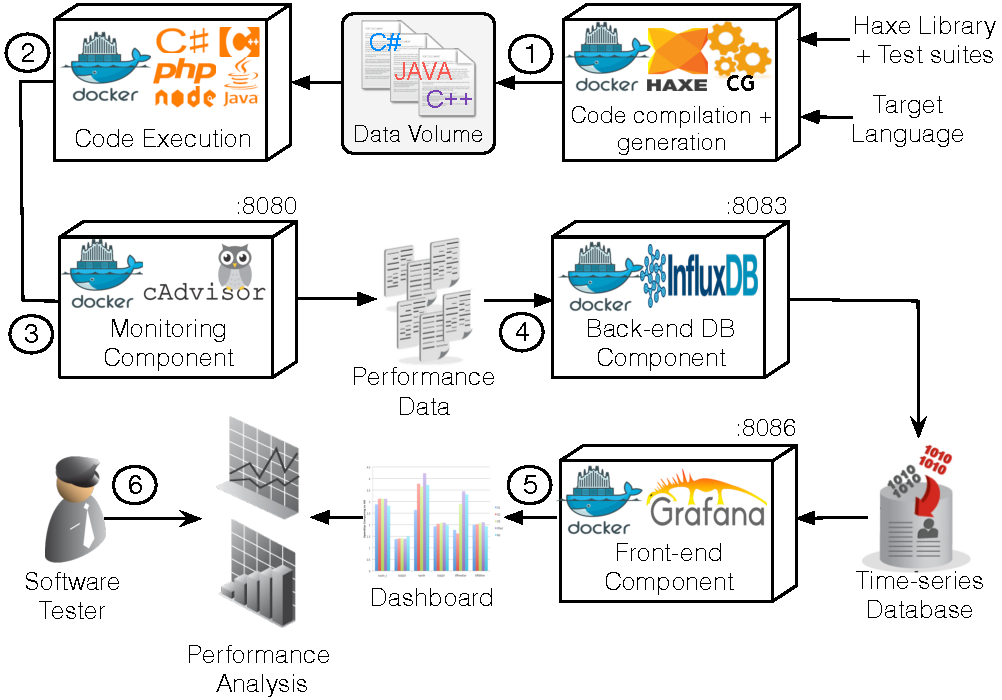
\includegraphics[width=1\linewidth]{Ressources/settingup.pdf}
	\caption{Infrastructure settings for running experiments}
\end{figure}
To assess our approach, we configure our previously proposed container-based infrastructure in order to run experiments on the Haxe case study.
Figure 3 shows a big picture of the testing and monitoring infrastructure considered in these experiments.


\begin{table}[h]
	\centering

	\resizebox{\columnwidth}{!}{%
	\begin{tabular}{|l|l|S[table-format=3.2]|l|S[table-format=3.2]|l|S[table-format=3.2]|}
		\hline
		\textbf{Benchmark}                 & \textbf{TestSuite} & \textbf{Std\_dev}                & \textbf{TestSuite} & \textbf{Std\_dev}             & \textbf{TestSuite} & \textbf{Std\_dev}              \\ \hline
		& \textbf{TS1}       & 0.55                             & \textbf{TS8}       & 0.24                          & \textbf{TS15}      & 0.73                           \\ \cline{2-7} 
		& \textbf{TS2}       & 0.29                             & \textbf{TS9}       & 0.22                          & \textbf{TS16}      & 0.12                           \\ \cline{2-7} 
		& \textbf{TS3}       & 0.34                             & \textbf{TS10}      & 0.10                          & \textbf{TS17}      & 0.31                           \\ \cline{2-7} 
		& \textbf{TS4}       & 2.51                             & \textbf{TS11}      & 0.17                          & \textbf{TS18}      & 0.34                           \\ \cline{2-7} 
		& \textbf{TS5}       & 1.53                             & \textbf{TS12}      & 0.28                          & \textbf{TS19}      & \cellcolor[HTML]{C0C0C0}120.61 \\ \cline{2-7} 
		& \textbf{TS6}       & 43.50                            & \textbf{TS13}      & 0.33                         & \multicolumn{2}{l|}{\multirow{2}{*}{}} \\ \cline{2-5}
		\multirow{-7}{*}{\textbf{Color}}   & \textbf{TS7}       & 0.50                             & \textbf{TS14}      & 1.88                          & \multicolumn{2}{l|}{}                  \\ \hline
		& \textbf{TS1}       & 0.35                             & \textbf{TS18}      & 0.16                          & \textbf{TS35}      & 1.30                           \\ \cline{2-7} 
		& \textbf{TS2}       & 0.07                             & \textbf{TS19}      & 0.60                          & \textbf{TS36}      & 1.13                           \\ \cline{2-7} 
		& \textbf{TS3}       & 0.30                             & \textbf{TS20}      & 5.79                          & \textbf{TS37}      & 2.02                           \\ \cline{2-7} 
		& \textbf{TS4}       & \cellcolor[HTML]{C0C0C0}27299.89 & \textbf{TS21}      & 0.47                          & \textbf{TS38}      & 0.26                           \\ \cline{2-7} 
		& \textbf{TS5}       & 6.12                             & \textbf{TS22}      & 2.74                          & \textbf{TS39}      & 0.16                           \\ \cline{2-7} 
		& \textbf{TS6}       & 21.90                            & \textbf{TS23}      & 2.14                          & \textbf{TS40}      & 8.12                           \\ \cline{2-7} 
		& \textbf{TS7}       & 0.41                             & \textbf{TS24}      & 3.79                          & \textbf{TS41}      & 5.45                           \\ \cline{2-7} 
		& \textbf{TS8}       & 0.28                             & \textbf{TS25}      & 0.19                          & \textbf{TS42}      & 0.11                           \\ \cline{2-7} 
		& \textbf{TS9}       & 0.78                             & \textbf{TS26}      & 0.13                          & \textbf{TS43}      & 1.41                           \\ \cline{2-7} 
		& \textbf{TS10}      & 1.82                             & \textbf{TS27}      & 5.59                          & \textbf{TS44}      & 1.56                           \\ \cline{2-7} 
		& \textbf{TS11}      & \cellcolor[HTML]{C0C0C0}180.68   & \textbf{TS28}      & 1.71                          & \textbf{TS45}      & 0.11                           \\ \cline{2-7} 
		& \textbf{TS12}      & \cellcolor[HTML]{C0C0C0}185.02   & \textbf{TS29}      & 0.26                          & \textbf{TS46}      & 1.04                           \\ \cline{2-7} 
		& \textbf{TS13}      & \cellcolor[HTML]{C0C0C0}128.78   & \textbf{TS30}      & 0.44                          & \textbf{TS47}      & 0.23                           \\ \cline{2-7} 
		& \textbf{TS14}      & 0.71                             & \textbf{TS31}      & 1.71                          & \textbf{TS48}      & 1.34                           \\ \cline{2-7} 
		& \textbf{TS15}      & 0.12                             & \textbf{TS32}      & 2.42                          & \textbf{TS49}      & 1.86                           \\ \cline{2-7} 
		& \textbf{TS16}      & 0.65                             & \textbf{TS33}      & 8.29                          & \textbf{TS50}      & 1.28                           \\ \cline{2-7} 
		\multirow{-17}{*}{\textbf{Core}}   & \textbf{TS17}      & 0.26                             & \textbf{TS34}      & 5.25                          & \textbf{TS51}      & 3.53                           \\ \hline
		& \textbf{TS1}       & 31.65                            & \textbf{TS3}       & 30.34                         & \textbf{TS5}       & 0.40                           \\ \cline{2-7} 
		\multirow{-2}{*}{\textbf{Hxmath}}  & \textbf{TS2}       & 4.27                             & \textbf{TS4}       & 0.25                          & \textbf{TS6}       & 0.87                           \\ \hline
		& \textbf{TS1}       & 0.28                             & \textbf{TS3}       & \cellcolor[HTML]{C0C0C0}95.36 & \textbf{TS4}       & 1.49                           \\ \cline{2-7} 
		\multirow{-2}{*}{\textbf{Format}}  & \textbf{TS2}       & \cellcolor[HTML]{C0C0C0}64.94    & \multicolumn{4}{l|}{\textbf{}}                                                                           \\ \hline
		\textbf{Promise}                   & \textbf{TS1}       & 0.29                             & \textbf{TS2}       & 13.21                         & \textbf{TS3}       & 1.21                           \\ \hline
		& \textbf{TS1}       & 0.13                             & \textbf{TS3}       & 0.13                          & \textbf{TS4}       & 1.40                           \\ \cline{2-7} 
		\multirow{-2}{*}{\textbf{Culture}} & \textbf{TS2}       & 0.10                             & \multicolumn{4}{l|}{}                                                                                    \\ \hline
		\textbf{Math}                      & \textbf{TS1}       & \cellcolor[HTML]{C0C0C0}642.85   & \textbf{TS2}       & 28.32                         & \textbf{TS3}       & 24.40                          \\ \hline
	\end{tabular}%
	}
 
		\caption{The comparison results of running each test suite across five target languages: the metric used is the standard deviation between execution times  }
 
 
 
		\label{my-label}
\end{table}

% Please add the following required packages to your document preamble:
% \usepackage{multirow}
% Please add the following required packages to your document preamble:
% \usepackage{multirow}
% \usepackage[table,xcdraw]{xcolor}
% If you use beamer only pass "xcolor=table" option, i.e. \documentclass[xcolor=table]{beamer}
\begin{table}[]
	\centering

	\resizebox{\columnwidth}{!}{%
	\begin{tabular}{|l|l|S[table-format=3.2]|l|S[table-format=3.2]|l|S[table-format=3.2]|}
		\hline
		\textbf{Benchmark}                 & \textbf{TestSuite} & \textbf{Std\_dev}               & \textbf{TestSuite} & \textbf{Std\_dev}              & \textbf{TestSuite} & \textbf{Std\_dev}              \\ \hline
		& \textbf{TS1}       & 10.19                           & \textbf{TS8}       & 1.23                           & \textbf{TS15}      & 14.44                          \\ \cline{2-7} 
		& \textbf{TS2}       & 1.17                            & \textbf{TS9}       & 1.95                           & \textbf{TS16}      & 1.13                           \\ \cline{2-7} 
		& \textbf{TS3}       & 0.89                            & \textbf{TS10}      & 1.27                           & \textbf{TS17}      & 0.72                           \\ \cline{2-7} 
		& \textbf{TS4}       & 30.34                           & \textbf{TS11}      & 0.57                           & \textbf{TS18}      & 0.97                           \\ \cline{2-7} 
		& \textbf{TS5}       & 31.79                           & \textbf{TS12}      & 1.11                           & \textbf{TS19}      & \cellcolor[HTML]{C0C0C0}777.32 \\ \cline{2-7} 
		& \textbf{TS6}       & \cellcolor[HTML]{C0C0C0}593.05  & \textbf{TS13}      & 0.46                           & \multicolumn{2}{l|}{}                               \\ \cline{2-5}
		\multirow{-7}{*}{\textbf{Color}}   & \textbf{TS7}       & 12.14                           & \textbf{TS14}      & 45.90                          & \multicolumn{2}{l|}{\multirow{-2}{*}{}}             \\ \hline
		& \textbf{TS1}       & 1.40                            & \textbf{TS18}      & 1.00                           & \textbf{TS35}      & 14.13                          \\ \cline{2-7} 
		& \textbf{TS2}       & 1.17                            & \textbf{TS19}      & 20.37                          & \textbf{TS36}      & 32.41                          \\ \cline{2-7} 
		& \textbf{TS3}       & 0.60                            & \textbf{TS20}      & 128.23                         & \textbf{TS37}      & 22.72                          \\ \cline{2-7} 
		& \textbf{TS4}       & \cellcolor[HTML]{C0C0C0}403.15  & \textbf{TS21}      & 24.38                          & \textbf{TS38}      & 2.19                           \\ \cline{2-7} 
		& \textbf{TS5}       & 41.95                           & \textbf{TS22}      & 76.24                          & \textbf{TS39}      & 0.26                           \\ \cline{2-7} 
		& \textbf{TS6}       & 203.55                          & \textbf{TS23}      & 18.82                          & \textbf{TS40}      & 126.29                         \\ \cline{2-7} 
		& \textbf{TS7}       & 19.69                           & \textbf{TS24}      & 72.01                          & \textbf{TS41}      & 31.01                          \\ \cline{2-7} 
		& \textbf{TS8}       & 0.78                            & \textbf{TS25}      & 0.21                           & \textbf{TS42}      & 0.93                           \\ \cline{2-7} 
		& \textbf{TS9}       & 30.41                           & \textbf{TS26}      & 2.30                           & \textbf{TS43}      & 50.36                          \\ \cline{2-7} 
		& \textbf{TS10}      & 57.19                           & \textbf{TS27}      & 101.53                         & \textbf{TS44}      & 12.56                          \\ \cline{2-7} 
		& \textbf{TS11}      & 68.92                           & \textbf{TS28}      & 43.67                          & \textbf{TS45}      & 0.91                           \\ \cline{2-7} 
		& \textbf{TS12}      & 74.19                           & TS29               & 0.90                           & \textbf{TS46}      & 27.28                          \\ \cline{2-7} 
		& \textbf{TS13}      & 263.99                          & \textbf{TS30}      & 4.02                           & \textbf{TS47}      & 1.10                           \\ \cline{2-7} 
		& \textbf{TS14}      & 19.89                           & \textbf{TS31}      & 52.35                          & \textbf{TS48}      & 15.40                          \\ \cline{2-7} 
		& \textbf{TS15}      & 0.30                            & \textbf{TS32}      & 134.75                         & \textbf{TS49}      & 37.01                          \\ \cline{2-7} 
		& \textbf{TS16}      & 28.29                           & \textbf{TS33}      & 82.66                          & \textbf{TS50}      & 23.29                          \\ \cline{2-7} 
		\multirow{-17}{*}{\textbf{Core}}            & \textbf{TS17}      & 1.16                            & \textbf{TS34}      & 89.57                          & \textbf{TS51}      & 1.28                           \\ \hline
		& \textbf{TS1}       & \cellcolor[HTML]{C0C0C0}444.18  & \textbf{TS3}       & \cellcolor[HTML]{C0C0C0}425.65 & \textbf{TS5}       & 17.69                          \\ \cline{2-7} 
		\multirow{-2}{*}{\textbf{Hxmath}}  & \textbf{TS2}       & 154.80                          & \textbf{TS4}       & 0.96                           & \textbf{TS6}       & 46.13                          \\ \hline
		& \textbf{TS1}       & 0.74                            & \textbf{TS3}       & 255.36                         & \textbf{TS4}       & 8.40                           \\ \cline{2-7} 
		\multirow{-2}{*}{\textbf{Format}}  & \textbf{TS2}       & 106.87                          & \multicolumn{4}{l|}{\textbf{}}                                                                            \\ \hline
		\textbf{Promise}                   & \textbf{TS1}       & 0.30                            & \textbf{TS2}       & 58.76                          & \textbf{TS3}       & 20.04                          \\ \hline
		& \textbf{TS1}       & 1.28                            & \textbf{TS3}       & 0.58                           & \textbf{TS4}       & 15.69                          \\ \cline{2-7} 
		\multirow{-2}{*}{\textbf{Culture}} & \textbf{TS2}       & 4.51                            & \multicolumn{4}{l|}{}                                                                                     \\ \hline
		\textbf{Math}                      & \textbf{TS1}       & \cellcolor[HTML]{C0C0C0}1041.53 & \textbf{TS2}       & 234.93                         & \textbf{TS3}       & 281.12                         \\ \hline
	\end{tabular}%
}
 
	\caption{The comparison results of running each test suite across five target languages: the metric used is the standard deviation between memory consumptions}
 
 

	\label{my-label}
\end{table}



\begin{table*}[h]
	\centering
	
	\resizebox{0.75\linewidth}{!}{%
		\begin{tabular}{|l|S[table-format=3.2]|S[table-format=3.2]|S[table-format=3.2]|S[table-format=3.2]|S[table-format=3.2]|S[table-format=3.2]|S[table-format=3.2]|S[table-format=3.2]|S[table-format=3.2]|S[table-format=3.2]|}
			\hline
			\multirow{2}{*}{}    & \multicolumn{2}{c|}{\textbf{JS}}   & \multicolumn{2}{c|}{\textbf{JAVA}} & \multicolumn{2}{c|}{\textbf{C++}}  & \multicolumn{2}{c|}{\textbf{CS}}   & \multicolumn{2}{c|}{\textbf{PHP}}  \\ \cline{2-11} 
			& \textbf{Time} & \textbf{Factor} & \textbf{Time} & \textbf{Factor} & \textbf{Time} & \textbf{Factor} & \textbf{Time} & \textbf{Factor} & \textbf{Time} & \textbf{Factor} \\ \hline
			\textbf{Color\_TS19} & 4.52             & x1.0            & 8.61             & x1.9            & 10.73            & x2.4            & 14.99            & x3.3            & 279.27           & x61.8           \\ \hline
			\textbf{Core\_TS4}   & 665.78           & x1.0            & 416.85           & x0.6            & 699.11           & x1.1            & 1161.29          & x1.7            & 61777.21         & x92.8           \\ \hline
			\textbf{Core\_TS11}  & 4.27             & x1.0            & 1.80             & x0.4            & 1.57             & x0.4            & 5.71             & x1.3            & 407.33           & x95.4           \\ \hline
			\textbf{Core\_TS12}  & 4.71             & x1.0            & 2.06             & x0.4            & 1.60             & x0.3            & 5.36             & x1.1            & 417.14           & x88.6           \\ \hline
			\textbf{Core\_TS13}  & 6.26             & x1.0            & 5.91             & x0.9            & 11.04            & x1.8            & 14.14            & x2.3            & 297.21           & x47.5           \\ \hline
			\textbf{Format\_TS2}   & 2.31             & x1.0            & 2.10             & x0.9            & 1.81             & x0.8            & 6.08             & x2.6            & 148.24           & x64.1           \\ \hline
			\textbf{Format\_TS3}   & 5.40             & x1.0            & 5.03             & x0.9            & 7.67             & x1.4            & 12.38            & x2.3            & 220.76           & x40.9           \\ \hline
			\textbf{Math\_TS1}   & 3.01             & x1.0            & 12.51            & x4.2            & 16.30            & x5.4            & 14.14            & x4.7            & 1448.90          & x481.7          \\ \hline
		\end{tabular}%
	}
	\caption{Raw data values of test suites that led to the highest variation in terms of execution time}
	\label{my-label}
\end{table*}


\begin{table*}[h]
	\centering

	\resizebox{0.75\linewidth}{!}{%
	\begin{tabular}{|l|S[table-format=3.2]|S[table-format=3.2]|S[table-format=3.2]|S[table-format=3.2]|S[table-format=3.2]|S[table-format=3.2]|S[table-format=3.2]|S[table-format=3.2]|S[table-format=3.2]|S[table-format=3.2]|}
		\hline
		\multirow{2}{*}{}    & \multicolumn{2}{c|}{\textbf{JS}}      & \multicolumn{2}{c|}{\textbf{JAVA}}    & \multicolumn{2}{c|}{\textbf{C++}}     & \multicolumn{2}{c|}{\textbf{CS}}      & \multicolumn{2}{c|}{\textbf{PHP}}     \\ \cline{2-11} 
		& \textbf{Memory} & \textbf{Factor} & \textbf{Memory} & \textbf{Factor} & \textbf{Memory} & \textbf{Factor} & \textbf{Memory} & \textbf{Factor} & \textbf{Memory} & \textbf{Factor} \\ \hline
		\textbf{Color\_TS6}  & 900.70              & x1.0            & 1362.55              & x1.5            & 2275.49             & x2.5            & 1283.31             & x1.4            & 758.79              & x0.8            \\ \hline
		\textbf{Color\_TS19} & 253.01              & x1.0            & 819.92              & x3.2            & 923.99              & x3.7            & 327.61              & x1.3            & 2189.86             & x8.7            \\ \hline
		\textbf{Core\_TS4}   & 303.09              & x1.0            & 768.22              & x2.5            & 618.42              & x2              & 235.75              & x0.8            & 1237.15             & x4.1            \\ \hline
		\textbf{Hxmath\_TS1} & 104.00              & x1.0            & 335.50              & x3.2            & 296.43              & x2.9            & 156.41              & x1.5            & 1192.98             & x11.5           \\ \hline
		\textbf{Hxmath\_TS3} & 111.68              & x1.0            & 389.73              & x3.5            & 273.12              & x2.4            & 136.49              & x1.2            & 1146.05             & x10.3           \\ \hline
		\textbf{Math\_TS1}   & 493.66              & x1.0            & 831.44              & x1.7            & 1492.97             & x3              & 806.33              & x1.6            & 3088.15             & x6.3            \\ \hline
	\end{tabular}%
}
	\caption{Raw data values of test suites that led to the highest variation in terms of memory usage}
	\label{my-label}
\end{table*}

 

First, we create a new Docker image in where we install the Haxe code generators and compilers (through the configuration file "Dockerfile"). Then a new instance of that image is created. It takes as an input the Haxe library we would to test and the list of test suites (step 1). It produces as an output the source code and binaries that have to be executed. These files are saved in a shared repository.
In Docker environment, this repository is called "data volume". A data volume is a specially-designated directory within containers that shares data with the host machine. So, when
we execute the generated test suites, we provide a shared volume with
the host machine so that, binaries can be executed in the execution container (Step 2). In fact, for the code execution we created, as well, a new Docker image in where we install all execution tools and environments such as php interpreter, NodeJS, etc. 

In the meantime, while running test suites inside the container, we collect runtime resource usage data using cAdvisor (step 3). The cAdvisor Docker image does not need any configuration on the host machine. We have just to run it on our host machine. It will then have access to resource usage and performance characteristics of all running containers. This image uses the Cgroups mechanism described previously to collect, aggregate, process, and export ephemeral real-time information about running containers. Then, it reports all statistics via web UI to view live resource consumption of each container. cAdvisor has been widely used in different projects such as Heapster\footnote{\url{https://github.com/kubernetes/heapster}} and Google Cloud Platform\footnote{\url{https://cloud.google.com/}}. In this experiment, we choose to gather information about the memory usage of running container.
Afterwards, we record these data into a new time-series database using our InfluxDB back-end container (step 4). %Thus, we define its corresponding ip port into the monitoring component so that, container statistics are sent over TCP port (e.g., \textit{8083}) exposed by the database component. 

Next, we run Grafana and we link it to InfluxDB. % by setting up the data source port 8086 so that, 
Grafana can  request data from the database. We recall that InfluxDB also provides a web UI to query the database and show graphs (step 5). But, Grafana let us display live results over time in much pretty looking graphs. Same as InfluxDB, we use SQL queries to extract non-functional metrics from the database for visualization and analysis (step 6). In our experiment, we are gathering the maximum memory usage values without presenting the graphs of resource usage profiles.

To obtain comparable and reproducible results, we use the same hardware across all experiments: a farm of AMD A10-7700K APU Radeon(TM) R7 Graphics processor with 4 CPU cores (\SI{2.0}{\GHz}), running Linux with a 64 bit kernel and \SI{16}{\giga\byte} of system memory. We reserve one core and \SI{4}{\giga\byte} of memory for each running container. 

\subsection{Experimental Results}
\subsubsection{Evaluation using the standard deviation}
We now conduct experiments based on the Haxe benchmark. We run each test suite 1K times and we report the execution time and memory usage across the different target languages: Java, JS, C++, CS, and PHP. 
The goal of running these experiments is to observe and compare the behavior of generated code regarding the testing load. We recall, as mentioned in the motivation, that we are not using any oracle function to detect inconsistencies. However, we rely on the comparison results across different targets to define code generator inconsistencies.
Thus, we use, as a quality metric, the standard deviation to quantify the amount of variation among execution traces (i.e., memory usage or execution time) and that for the five target languages. We recall that the formula of standard deviation is the square root of the variance. Thus, we are calculating this variance as the squared differences from the mean. Our data values in our experiment represent the obtained values in five languages. So, for each test suite we are taking the mean of these five values in order to calculate the variance.
A low standard deviation of a test suite execution, indicates that the data points (execution time or memory usage data) tend to be close to the mean which we consider as an acceptable behavior.  
On the other hand, a high standard deviation indicates that one or more data points are spread out over a wider range of values which can be more likely interpreted as a code generator inconsistency. 



In Table 3, we report the comparison results of running the benchmark in terms of execution speed. At the first glance, we can clearly see that all standard deviations are more mostly close to 0 - 8 interval. It is completely normal to get such small deviations, because we are comparing the execution time of test suites that are written in heterogeneous languages and executed using different technologies (e.g., interpreters for PHP, JVM for JAVA, etc.). So, it is expected to get a small deviation between the execution times after running the test suite in different languages. However, we remark in the same table, that there are some variation points where the deviation is relatively high. We count 8 test suites where the deviation is higher than 60 (highlighted in gray). We choose this value (i.e., standard deviation = 60) as a threshold to designate the points where the variation is extremely high. Thus, we consider values higher than 60 as a potential possibility that a non-functional bug could occur. These variations can be explained by the fact that the execution speed of one or more test suites varies considerably from one language to another. This argues the idea that the code generator has produced a suspect behavior of code for one or more target language. We provide later better explanation in order to detect the faulty code generators.

Similarly, Table 4 resumes the comparison results of test suites execution regarding memory usage. The variation in this experiment are more important than previous results. This can be argued by the fact that the memory utilization and allocation patterns are different for each language. Nevertheless, we can recognize some points where the variation is extremely high. Thus, we choose a threshold value equal to 400 and we highlighted, in gray, the points that exceed this threshold. Thus, we detect 6 test suites where the variation is extremely high. 
One of the reasons that caused this variation may occur when the test suite executes some parts of the code (in a specific language) that are so greedy in terms of resources. This may be not the case when the variation is lower than 10 for example.
We assume then that the faulty code generator, in this case, represents a threat for software quality since it can generate a code that is very resource consuming.
 
The inconsistencies we are trying to find here are more related to the incorrect memory utilization patterns produced by the faulty code generator. Such inconsistencies may come from an inadequate type usage, high resource instantiation, etc.





\subsubsection{Analysis}
Now that we have observed the non-functional behavior of test suites execution in different languages, we can analyze the extreme points we have detected in previous tables to observe more in deep the source of such deviation.
For that reason, we present in Table 5 and 6 the raw data values of these extreme test suites in terms of execution time and memory usage. 

Table 5 is showing the execution time of each test suite in a specific target language. We provide also factors of execution times among test suites running in different languages by taking as a baseline the JS version. 
We can clearly see that the PHP code has can have a singular behavior regarding the performance with a factor ranging from x40.9 for test suite 3 in benchamrk Format (Format\_TS3) to x481.7 for Math\_TS1. We remark also that running Core\_TS4 takes 61777 seconds (almost 17 hours) compared to a 416 seconds (around 6 minutes) in JAVA which is a very large gap. The highest factor detected for other languages ranges from x0.3 to x5.4 which is not negligible but it represents a small deviation compared to PHP version. While it is true that we are comparing different versions of generated code, it was expected to get some variations while running test cases in terms of execution time. However, in the case of PHP code generator it is far to be a simple variation but it is more likely to be a code generator inconsistency that led to such performance regression.


Meanwhile, we gathered information about the points that led to the highest standard deviation in terms of memory usage. Table~6 shows these results. %We take as well the JS version as a baseline since it requires less memory. 
Again, we can identify singular behavior regarding the performance. For Color\_TS6, C\# version consumes the highest memory (x2.5 more than JS). For other test suites versions, the factor varies from x0.8 to x3.7. %Besides the performance issues of PHP code generator presented in table~5, the results of memory usage confirm our claim since the PHP code has the highest memory utilization.
 
Focusing particularly on the singular performance of PHP code in core TS4, we observe the intensive use of \textit{"arrays"} in most of the functions under test. Arrays are known to be slow in PHP and PHP library has introduced many advanced functions such as $array\_fill$ and specialized abstract types such as \textit{"SplFixedArray"}\footnote{\url{http://php.net/manual/fr/class.splfixedarray.php}} to overcome this limitation. By changing just these two parts in the code generator, we improve the PHP code speed with a factor x5. 


In short, the lack of use of specific types, in native PHP standard library, by the PHP code generator such as \textit{SplFixedArray} shows a real impact on the non-functional behavior of generated code. In contrast, selecting carefully the adequate types and functions to generate code by code generators can lead to performance improvement.  We can observe the same kind of error in the C++ program  during one test suite execution (Color\_TS6) which consumes too much memory. The types used in the code generator are not the best ones. 

\subsection{Threats to Validity}
Any automated approach has limitations. We resume, in the following paragraphs, external and internal threats that can be raised:

\textit{External validity} refers to the generalizability of our findings. In this study, we perform experiments on Haxe and a set of test suite selected from Github and from the Haxe community. We have no guarantee that these libraries covers all the Haxe language features neither than all the Haxe standard libraries. Consequently, we cannot guarantee that the approach is able to find all the code generators issues. In particular, the threshold to detect singular behavior has a huge impact on the precision and recall of the proposed approach. Experiments should be replicated to other case studies to confirm our findings and try to understand the best heuristic to detect the code generator issues regarding performance. 

\textit{Internal validity} is concerned with the use of a container-based approach. Even if it exists emulator such as Qemu that allows to reflect the behavior of heterogeneous hardware, the chosen infrastructure has not been evaluated to test generated code that target heterogeneous hardware machine. In such a case, the provided compiler for a dedicated hardware can provide specific optimizations that lead to a large number of false positives. 
 


%hrough these conducted experiments, we reached interesting results, some of which were unexpected.


%In most languages, arrays are fixed-sized, but this is not the case in PHP since they are allocated dynamically. The dynamic allocation of arrays  leads to a slower write time because the memory locations needed to hold the new data is not already allocated. Thus, slow writing speed damages the performance of PHP code and impact the memory usage. This observation clearly confirm our early findings. The solution for this problem may be to use another type of object from the Standard PHP Library. As an alternative, \textit{"SplFixedArray"} pre-allocates the necessary memory and allows a faster array implementation, thereby solving the issue of slower write times. [ref to spl benchs]

%\subsection{Discussions}
%For instance, the poor performance of the Haxe-produced PHP code was certainly a surprise. 
%The PHP target had a very large execution time and memory usage for almost every test suite execution. 
%That is to say that PHP code generator is clearly generating non-efficient code regarding the non-functional properties. It is even possible to say that other code generators are not extremely efficient since we found that C++ code consumed, during one test suite execution (Color\_TS6), more memory than PHP. But, we cannot say for sure that C++ code generator is buggy. Thus, we cannot make any assumption. Nevertheless, the only point which, at this stage, can be statistically made is that PHP code generator has a real performance issue that has to be fixed by code generators developers. 

%In attempting to understand the reasons of this PHP performance issues, we tried to take a look at the source code generated in PHP. As an example, we looked at the source code of Core\_TS4. 





 







\section{Related Work}
//The idea of employing container-based approach for testing code generators can be found in several publications.

Previous work on non-functional testing of code generators focuses on comparing, as oracle, the non-functional properties of hand-written code to automatically generated code~\cite{stepasyuk2015evaluating,richard2013efficient}. As an example, Strekelj et al.~\cite{vstrekelj2015performance} implemented a simple 2D game in both the Haxe programming language and the native environment and evaluated the difference in performance between the two versions of code. They showed that the generated code through Haxe has better performance than hand-written code. 

Cross-platform mobile development has been also part of the non-functional testing goals since many code generators are increasingly used in industry for automatic cross-platform development. in \cite{pazirandeh2015evaluation,hartmann2011cross}, authors compare the performance of a set of cross-platform code generators and presented the most efficient tools.

Most of the previous work on code generators testing focuses on checking the correct functional behavior of generated code. Stuermer et al.~\cite{stuermer2007systematic} present a systematic test approach for model-based code generators. They investigate the impact of optimization rules for model-based code generation by comparing the output of the code execution with the output of the model execution. 
If these outputs are equivalent, it is assumed that the code generator works as expected. 
They evaluate the effectiveness of this approach by means of testing optimizations performed by the TargetLink code generator. 
They have used Simulink as a simulation environment of models. 

In \cite{jorges2014back}, authors presented a testing approach of the Genesys code generator framework which tests the translation performed by a code generator from a semantic perspective rather than just checking for syntactic correctness of the generation result.


In our approach, we provide a component-based infrastructure to compare non-functional properties of generated code rather than functional ones. 

\iffalse
Our work is related to iterative compilation research field.
The basic idea of iterative compilation is to explore the compiler optimization space by measuring the impact of optimizations on software performance.
Several research efforts have investigated this optimization problem to catch relevant optimizations regrading performance, energy or code size improvements over standard optimization sequences~\cite{almagor2004finding,hoste2008cole,pan2006fast,zhong2009tuning,pallister2015identifying,chen2012deconstructing,sandran2012genetic,martins2014exploration,fursin2008milepost,lin2008automatic,schulte2014post}. 
The vast majority of the work on iterative compilation focuses on increasing the speedup of new optimized code compared to standard optimizations. 
It has been proven that optimizations are highly dependent on target platform and input program. Compared to our proposal, we rather focus on comparing the resource consumption of optimized code.

Novelty Search has never been applied in the filed of iterative compilation. Our work presents the first attempt to introduce diversity in optimization sequences generation. The idea of NS has been introduced by Lehman et al.~\cite{lehman2008exploiting}. It has been often evaluated in deceptive tasks and especially applied to evolutionary robotics~\cite{risi2010evolving,krvcah2012solving} (in the context of neuroevolution). 
NS can easily be adapted to different research fields. In a previous work~\cite{boussaa2015novelty}, NS has been adapted for test data generation where novelty score was calculated as the Manhattan distance between the different vectors representing test data.
In our NS adaptation, we are measuring the novelty score using the systematic difference between optimization sequences of GCC.

For code generators testing, Stuermer et al.~\cite{stuermer2007systematic} present a systematic test approach for model-based code generators. They investigate the impact of optimization rules for model-based code generation by comparing the output of the code execution with the output of the model execution. 
If these outputs are equivalent, it is assumed that the code generator works as expected. 
They evaluate the effectiveness of this approach by means of testing optimizations performed by the TargetLink code generator. 
They have used Simulink as a simulation environment of models. 
In our approach, we provide a component-based infrastructure to compare non-functional properties of generated code rather than functional ones. 
\fi

\section{Conclusion and Future Work}

In this paper we have described a new approach for testing and monitoring code generators families using a container-based infrastructure. 
We used a set of micro-services in order to provide a fine-grained understanding of resource consumption. 
To validate the approach, we applied the proposed approach on an popular family of code generators: Haxe. 
The evaluation shows that the approach finds real issues in the existing code generators. 
In particular, we show that we could find two kinds of errors: the lack of use of a specific function and abstract type that exist in the standard library of a targeted language  that can reduce the memory/CPU consumption of the resulting program.

As a current work, we are discussing with the Haxe community to submit a patch with the first discoveries. 
We are also conducting the same evaluation for two other code generator families: ThingML and TypeScript. 
As a future work, we will improve our understanding on the threshold that provides a best precision for detecting performance issue in code generators. 




 

 
 

%\acks

%This work was funded by the European Union Seventh Framework Program (FP7/2007-2013) under grant agreement n611337, HEADS project (www.heads-project.eu)

% We recommend abbrvnat bibliography style.

\bibliographystyle{abbrvnat}

\bibliography{ref}

 
% The bibliography should be embedded for final submission.

 


\end{document}
